\subsection{Sun Scan}\label{sec:sun_scan}
We performed sun scans with two different settings.
A step size of \SI{0.5}{\degree} with a total scan width of \SI{20}{\degree} and a step size of \SI{0.1}{\degree} with a total scan width of \SI{10}{\degree}.
For each of the settings we performed a horizontal and a vertical scan centered around the sun.
The integrated power spectra are then each normalized by subtracting the minimum and then dividing by the resulting maximum.
These normalized values are shown in figure~\ref{fig:sun_scan}.
Measurements were performed on (02.10.2025, 11:20 - 11:40 MESZ), the sun was at Azimuth/Elevation of $\approx$ 145°/33°.

Recorded Data:
\begin{itemize}
    \item \path{Measurements/SunScan/SunScan_Az10deg_Res0deg5_T1120_20251002.hdf}
    \item \path{Measurements/SunScan/SunScan_Elv10deg_Res0deg5_T1120_20251002.hdf}
    \item \path{Measurements/SunScan/SunScan_Az5deg_Res0deg1_T1130_20251002.hdf}
    \item \path{Measurements/SunScan/SunScan_Elv5deg_Res0deg1_T1130_20251002.hdf}
\end{itemize}


\begin{figure}[H]
    \centering
    \begin{subfigure}[t]{0.45\linewidth}
        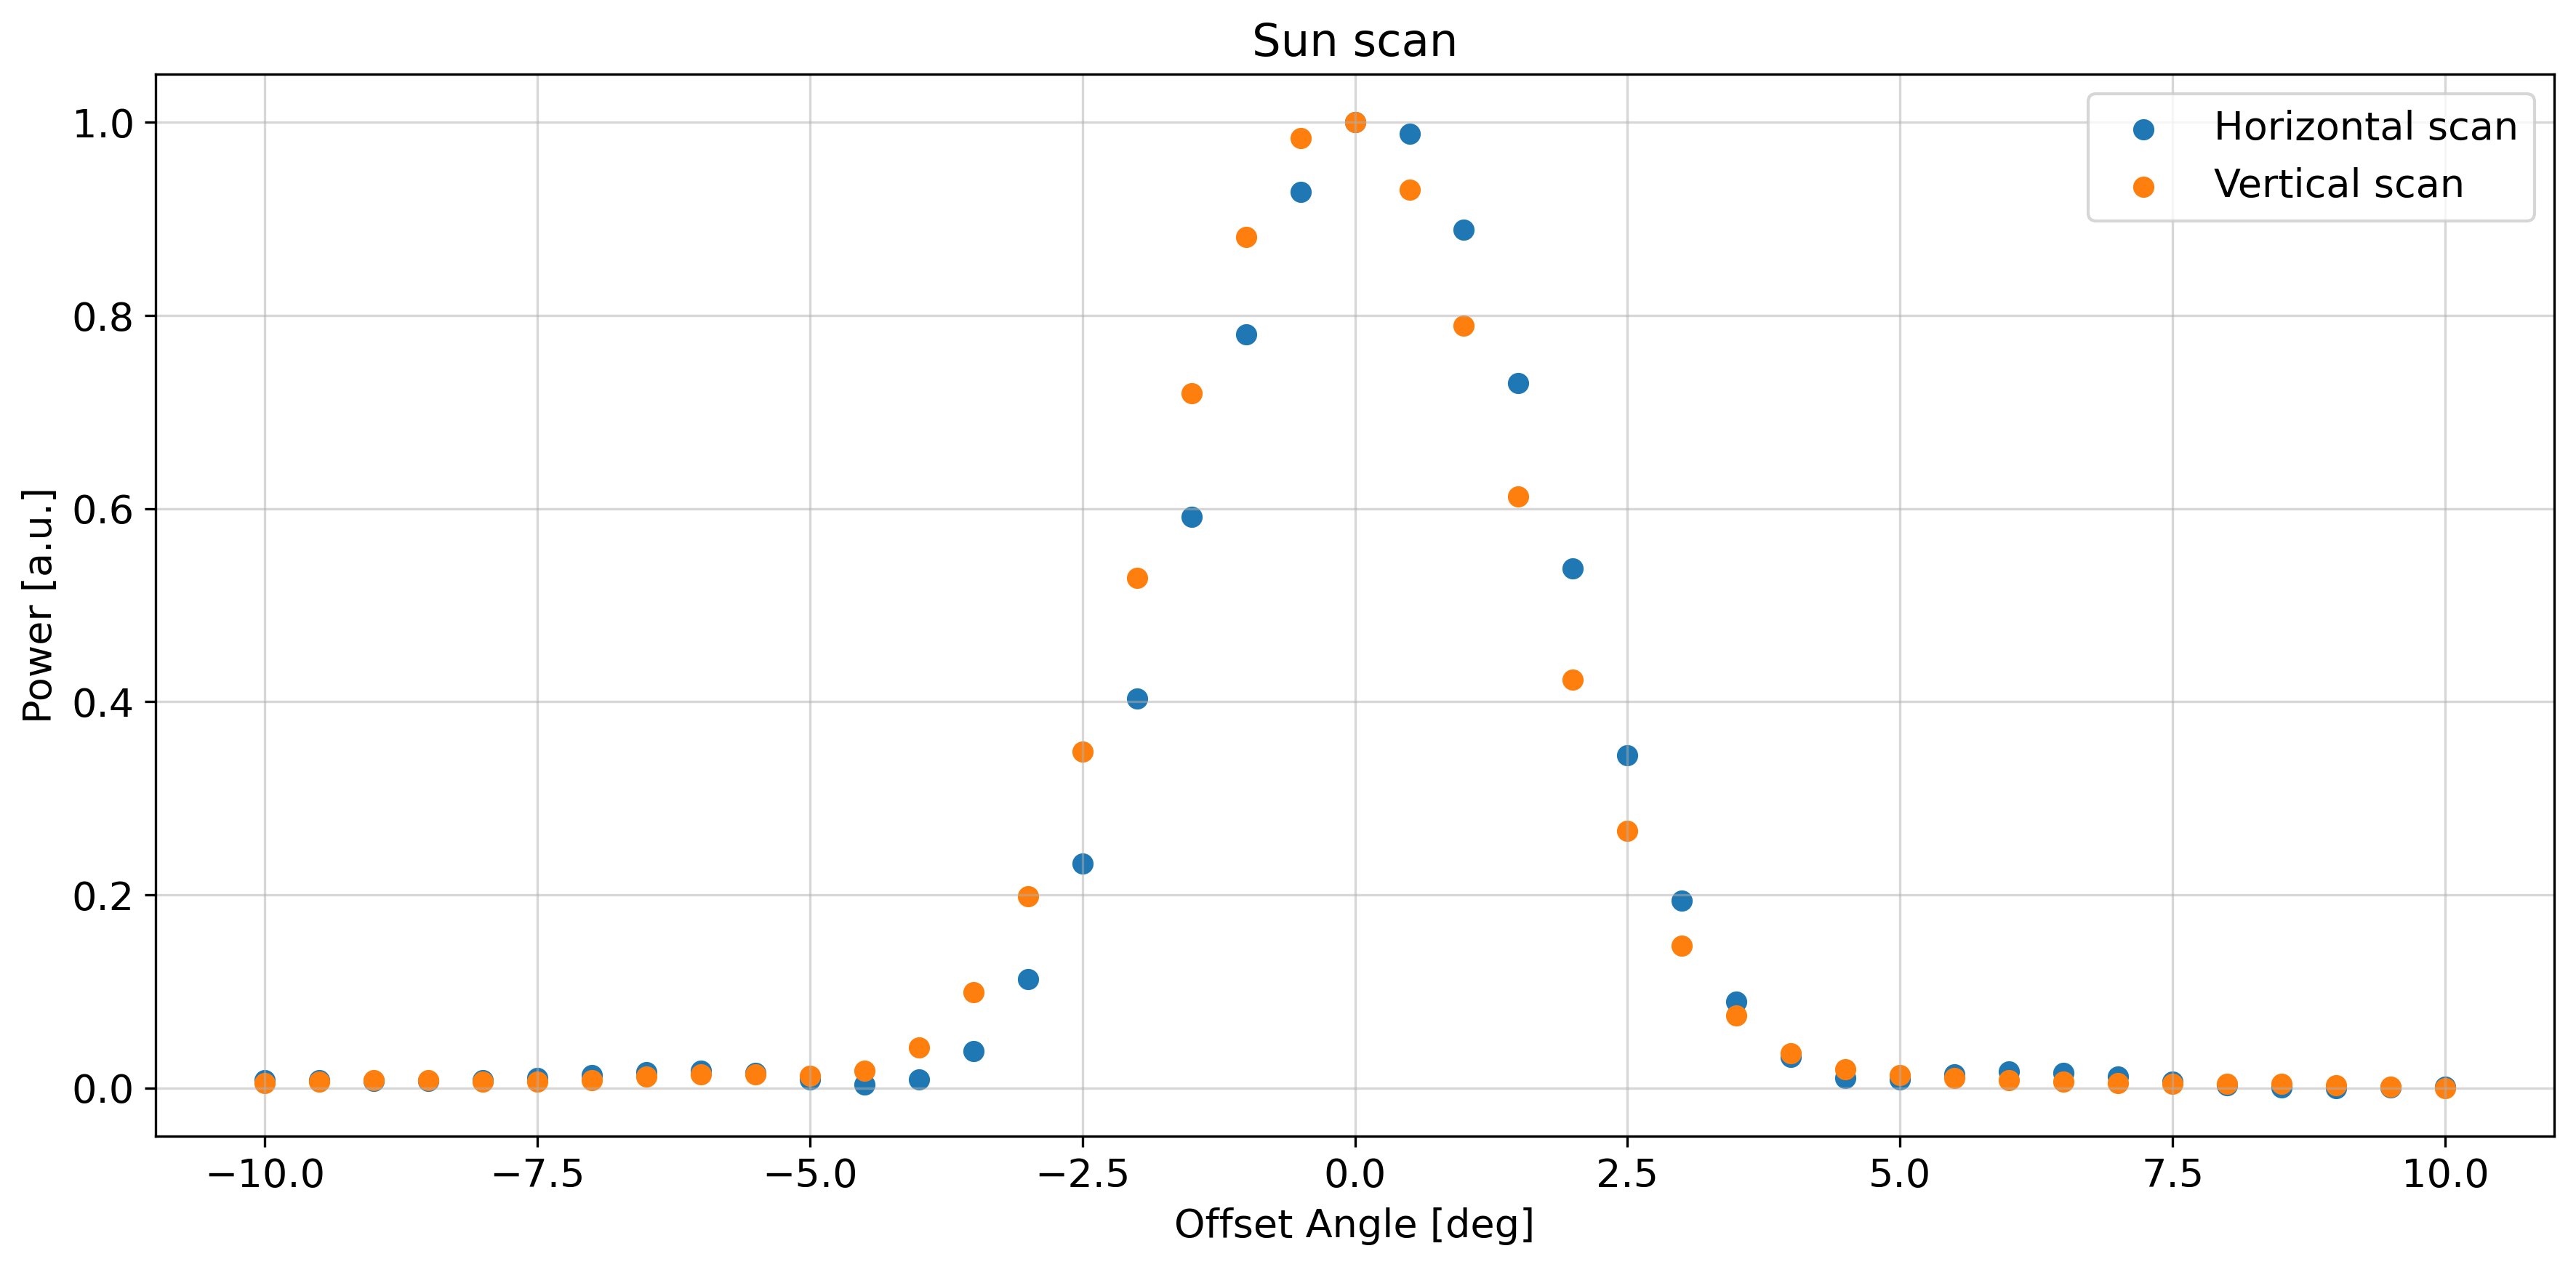
\includegraphics[width=\linewidth]{assets/sun_scan_low_res.png}
    \end{subfigure}
    \begin{subfigure}[t]{0.45\linewidth}
        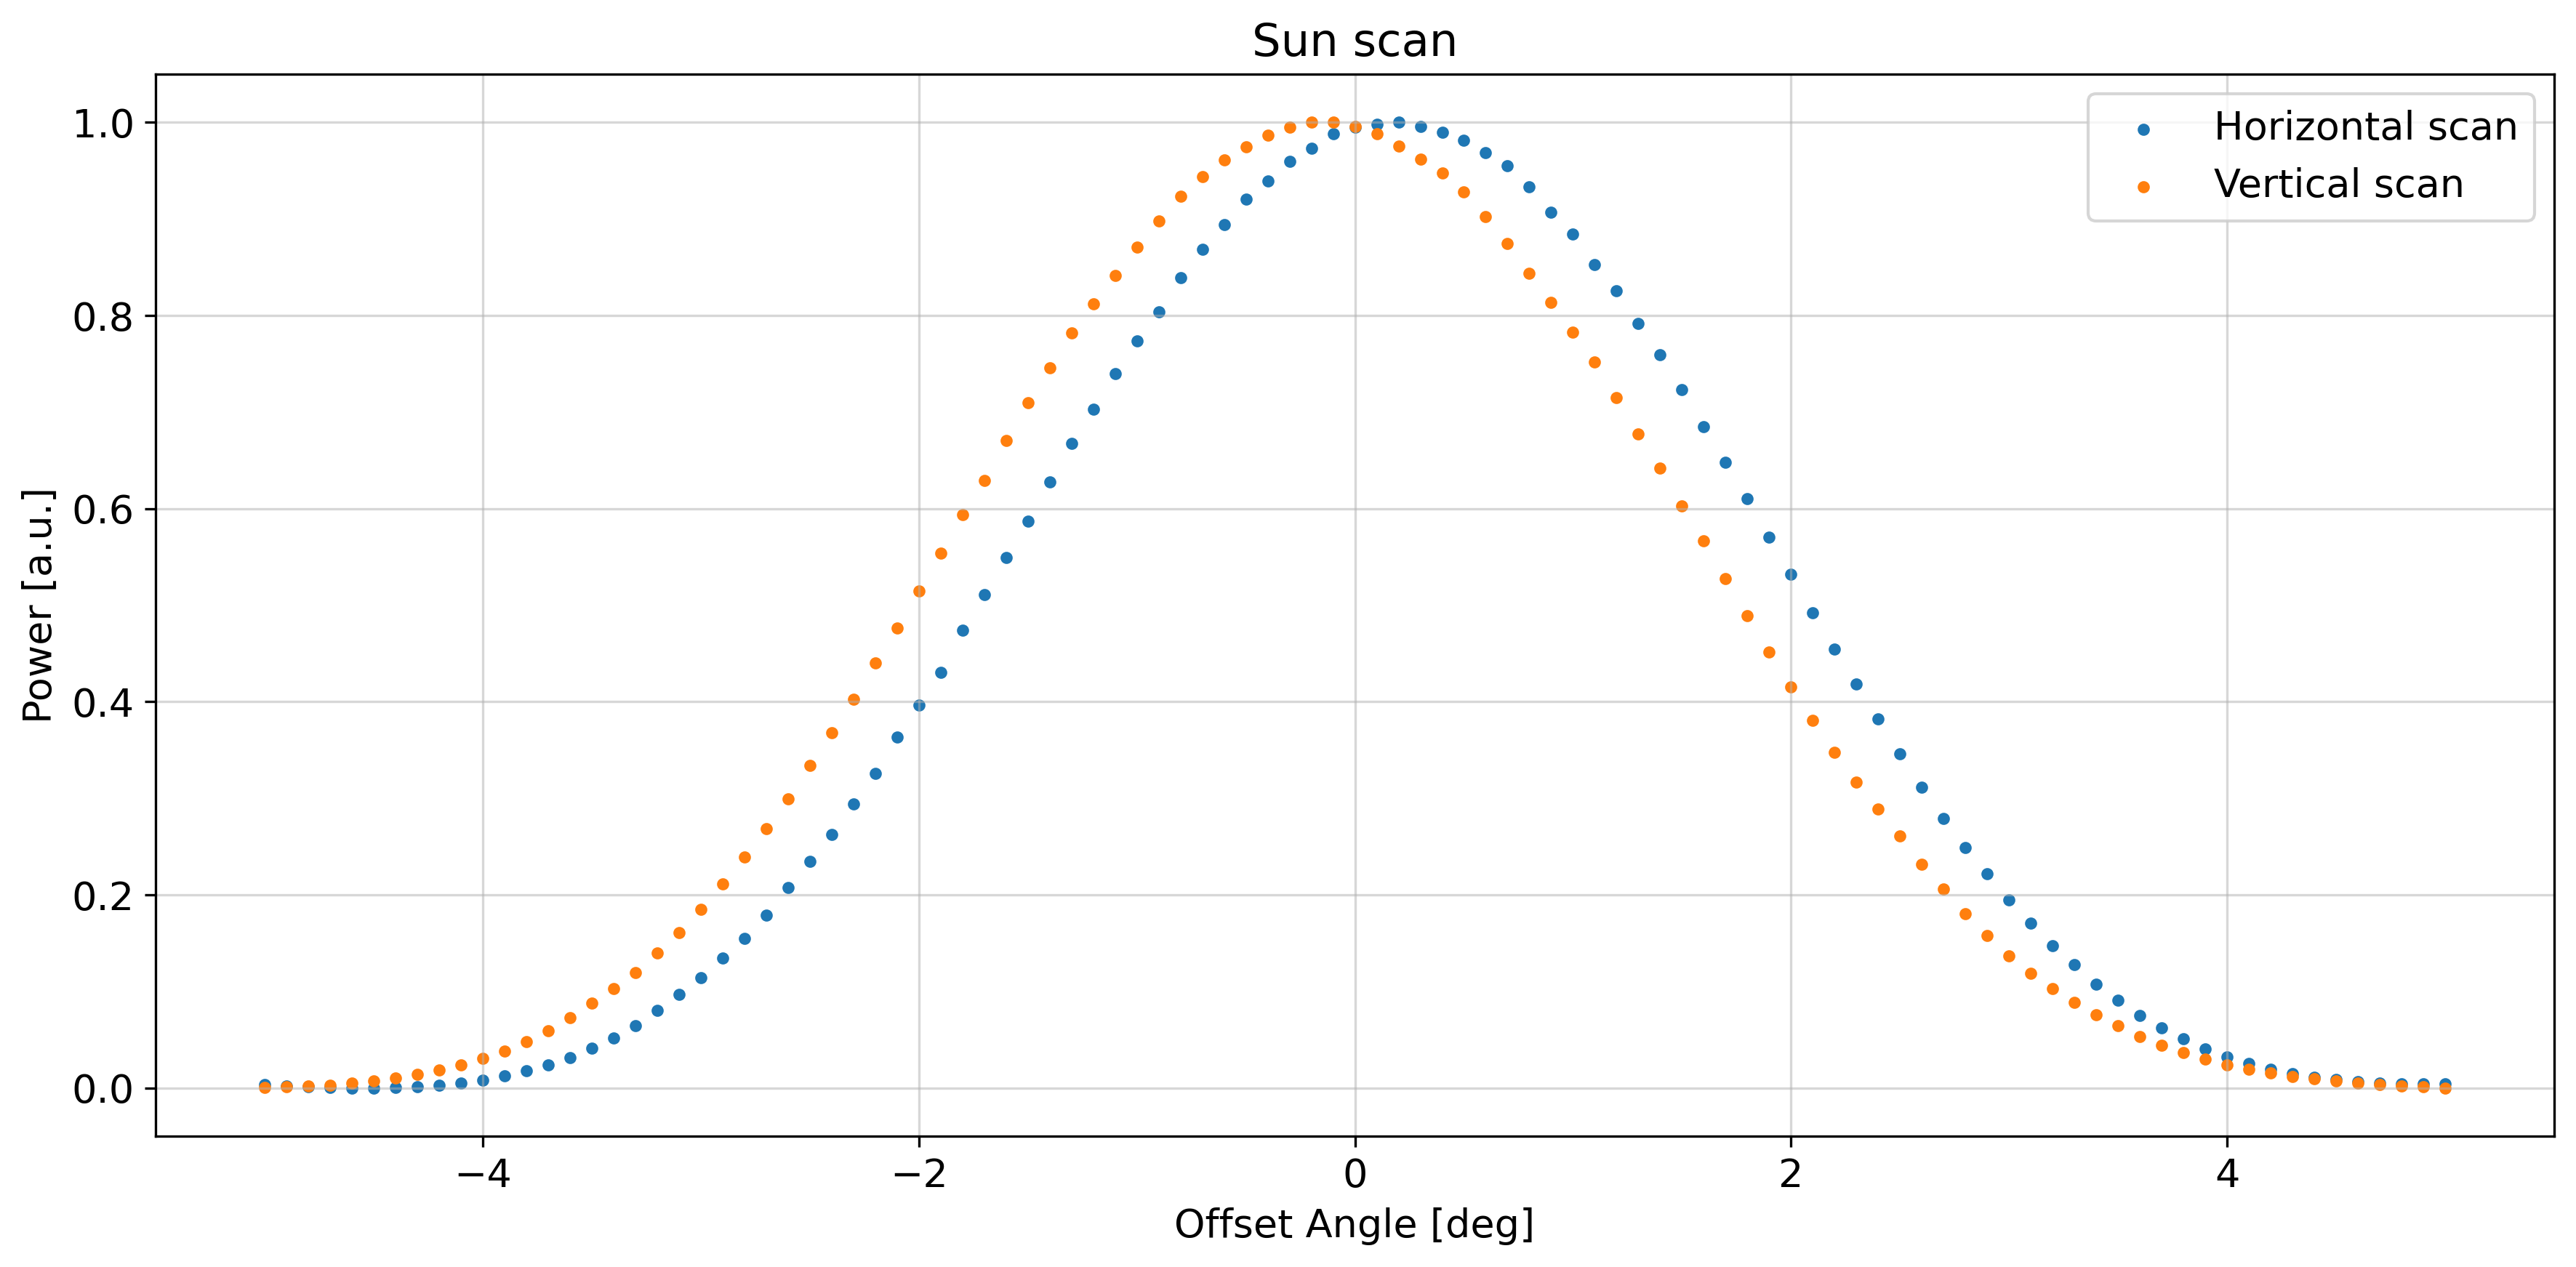
\includegraphics[width=\linewidth]{assets/sun_scan_high_res.png}
    \end{subfigure}
    \caption{Scan of the sun with a linear scale}
    \label{fig:sun_scan}
\end{figure}

The sidelobes are more visible when the normalized power is shown logarithmically, this is shown in figure~\ref{fig:sun_scan_log}
\begin{figure}[H]
    \centering
    \begin{subfigure}[t]{0.45\linewidth}
        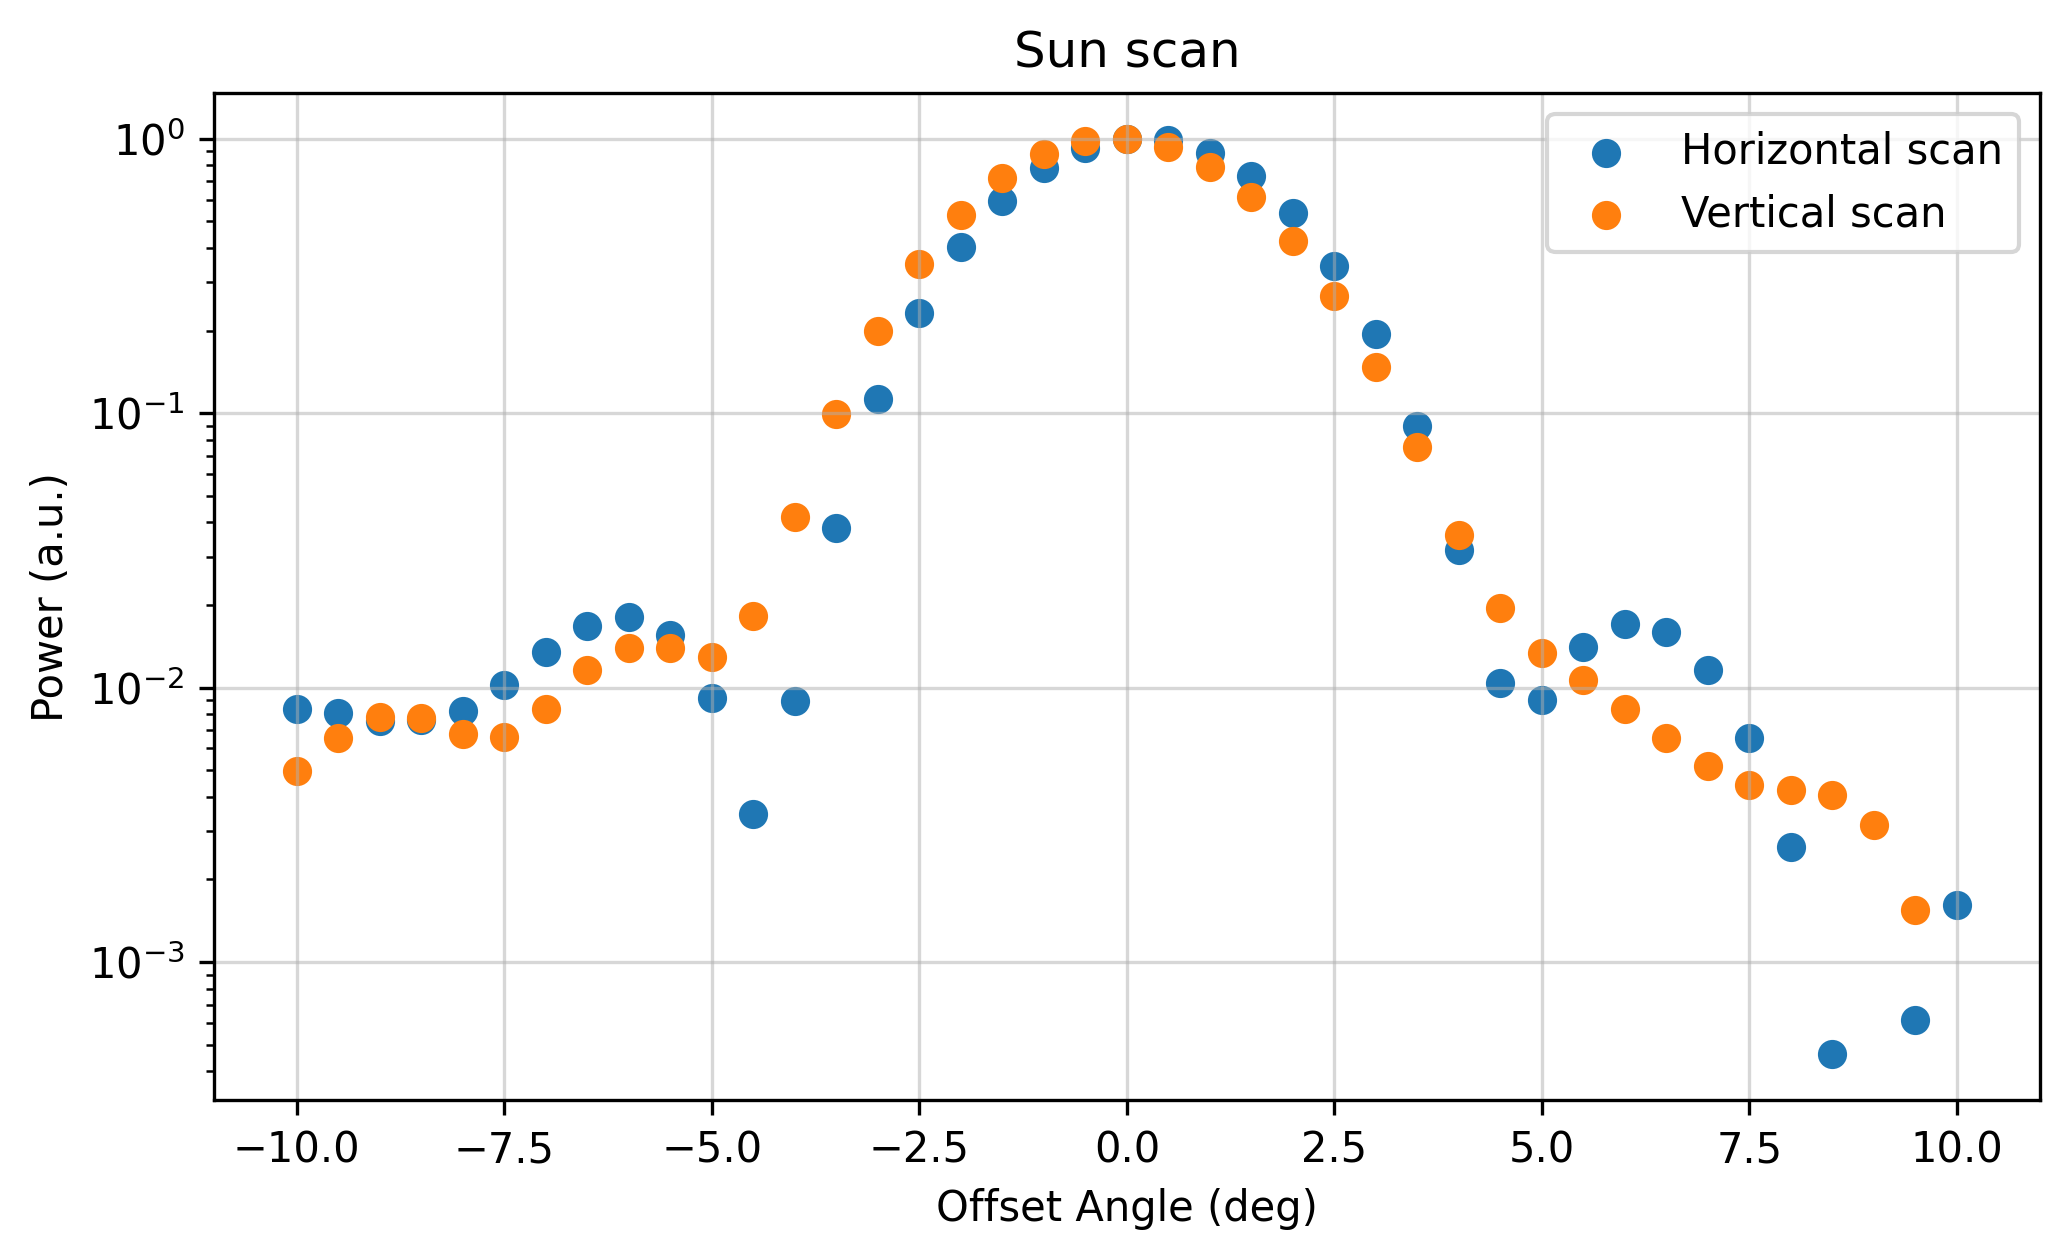
\includegraphics[width=\linewidth]{assets/sun_scan_low_res_log.png}
    \end{subfigure}
    \begin{subfigure}[t]{0.45\linewidth}
        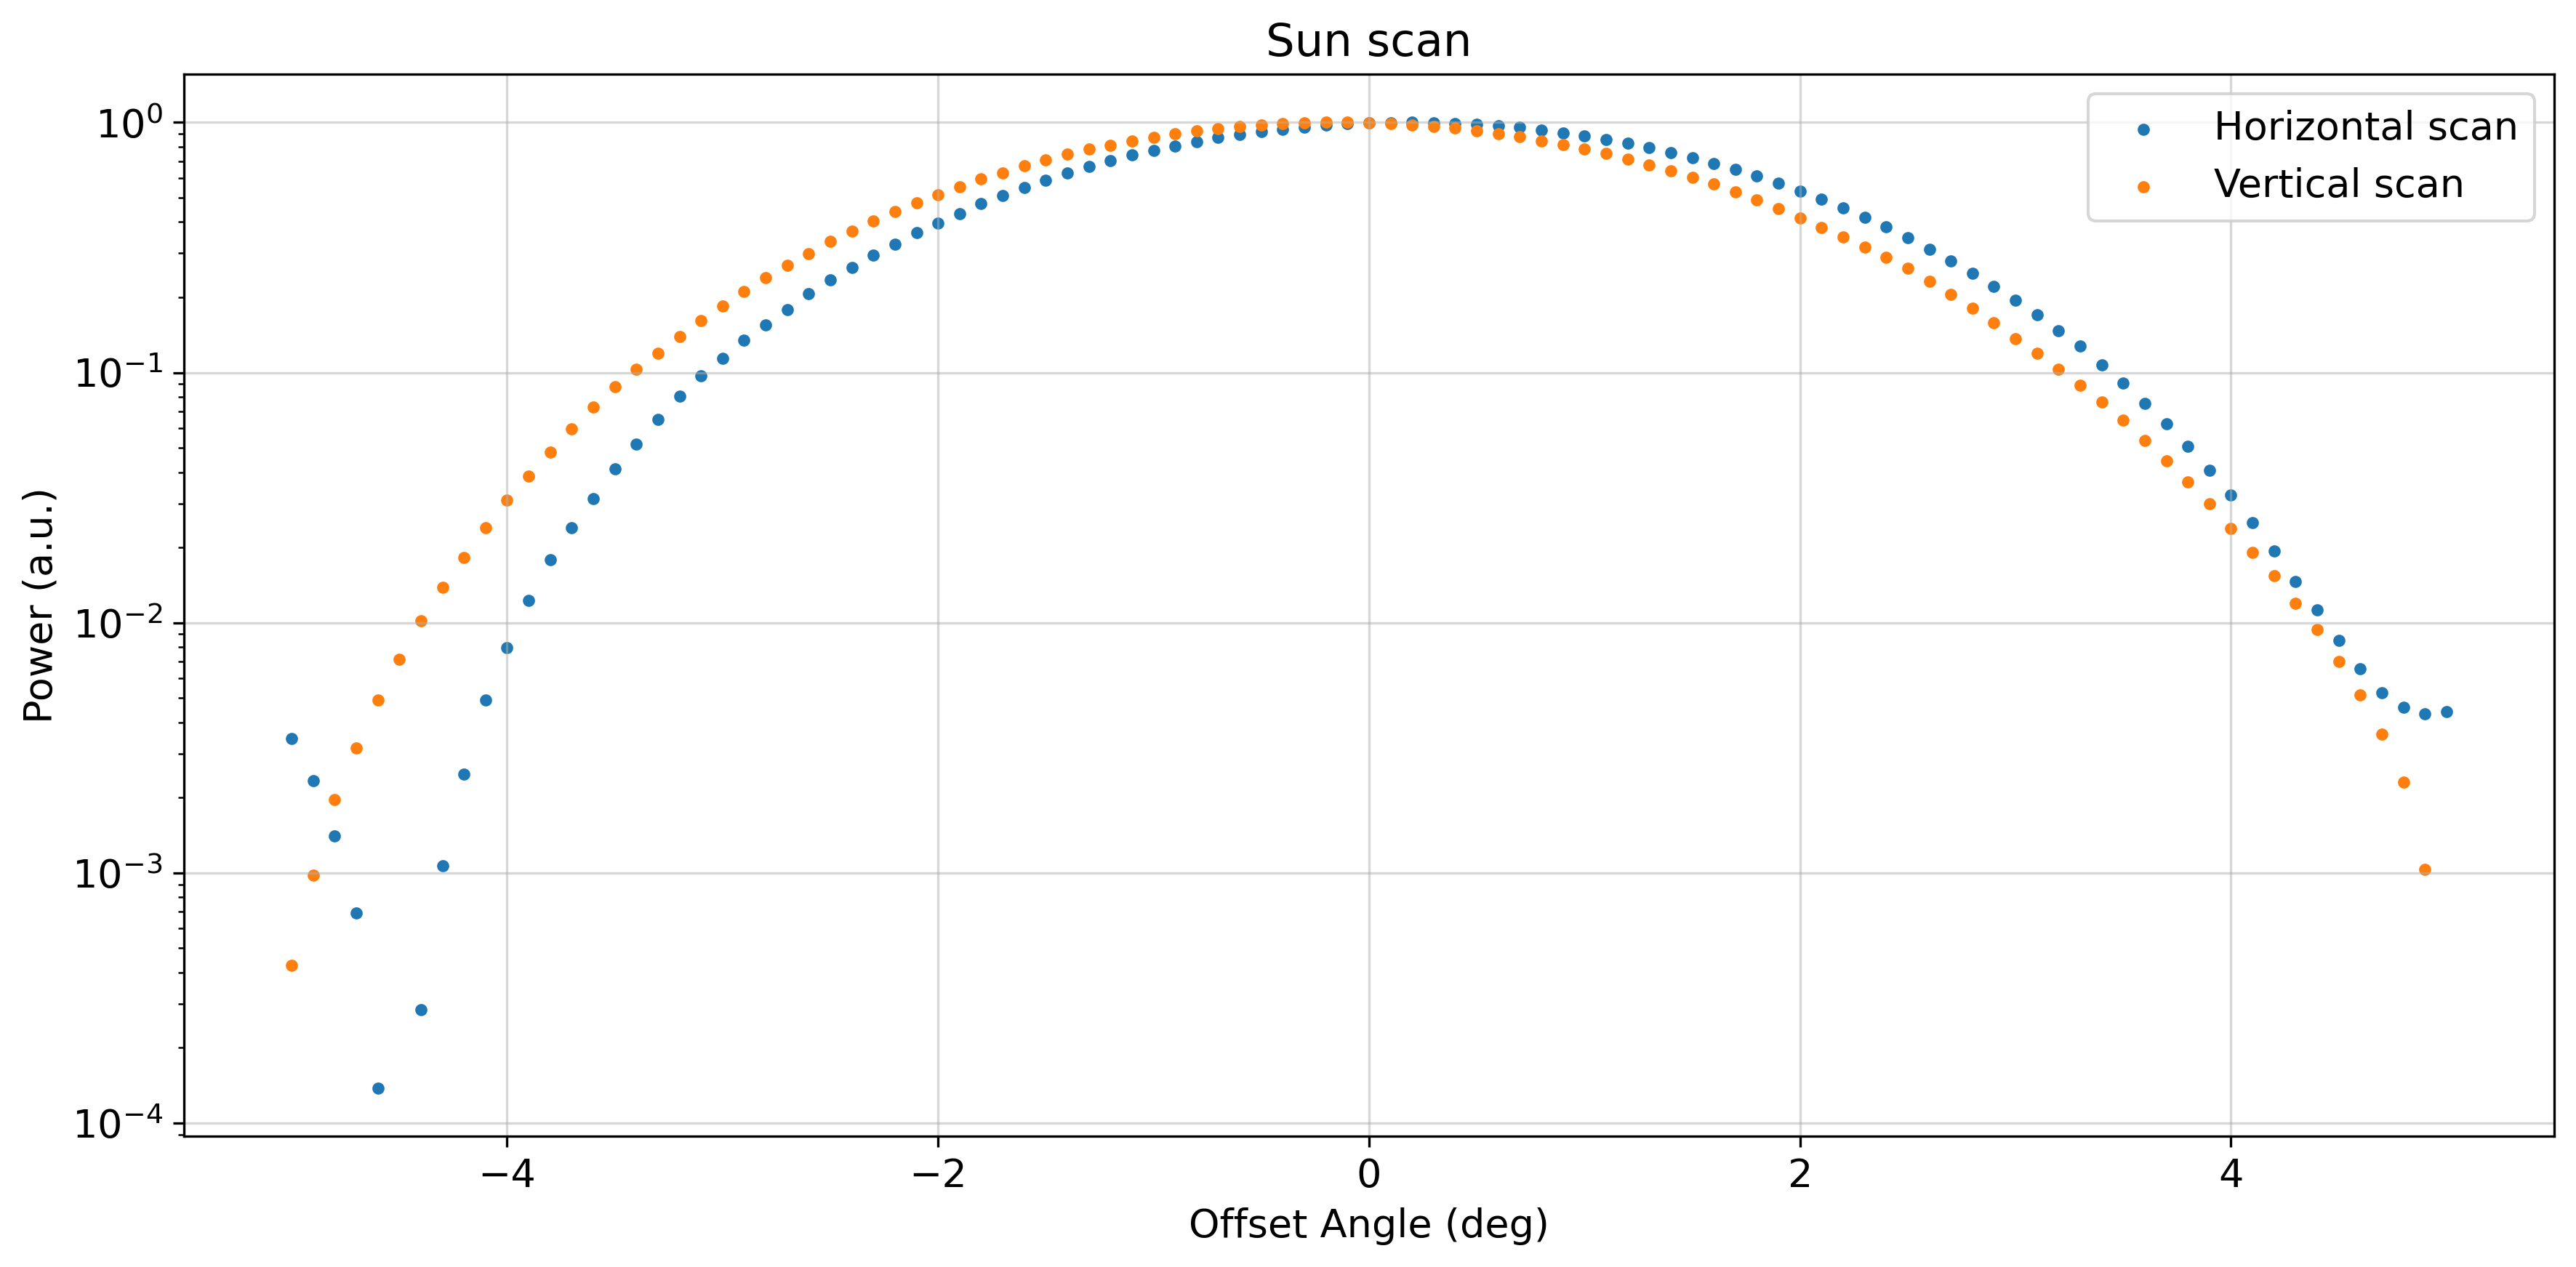
\includegraphics[width=\linewidth]{assets/sun_scan_high_res_log.png}
    \end{subfigure}
    \caption{Scan of the sun with a logarithmic scale}
    \label{fig:sun_scan_log}
\end{figure}

To determine the full width at half maximum (FWHM) we use the high resolution data and fit it to a gaussian.
The functional model is therefore described by the equation $f_{\theta_0, \sigma}(\theta)$.
\begin{equation}
    f_{\theta_0, \sigma}(\theta) = \exp{\left(-\frac{(\theta-\theta_0)^2}{2\sigma^2}\right)}
\end{equation}
The model can then be fitted using iterative least squares as described in \cite{ghilani_adjustment_2006} with initial guesses of $\theta_0 = 0$ and $\sigma = 1$. The FWHM can then be computed using Eq. \eqref{eq:fwhm_sigma}.
The resulting values are shown in table \ref{tab:params} and figure \ref{fig:sun_scan_fit}. The errors were computed statistically via the residual mean squared.

\begin{table}[H]
    \centering
    \begin{tabular}{lrrrr}
        \toprule
        Direction & FWHM [\si{\degree}] & $\sigma$  [\si{\degree}] & $\theta_0$ [\si{\degree}] & RMS $m_0$\\
        \midrule
        Horizontal & \SI{3.72(0.01)}{}   & \SI{1.581(0.005)}{} & \SI{ 0.179(0.006)}{} & 0.015\\
        Vertical   & \SI{3.751(0.009)}{} & \SI{1.593(0.004)}{} & \SI{-0.131(0.005)}{} & 0.011\\
        \bottomrule
    \end{tabular}
    \caption{functional model parameters from least squares fit}
    \label{tab:params}
\end{table}
\begin{figure}[H]
    \centering
    \begin{subfigure}[b]{0.45\textwidth}
        \centering
        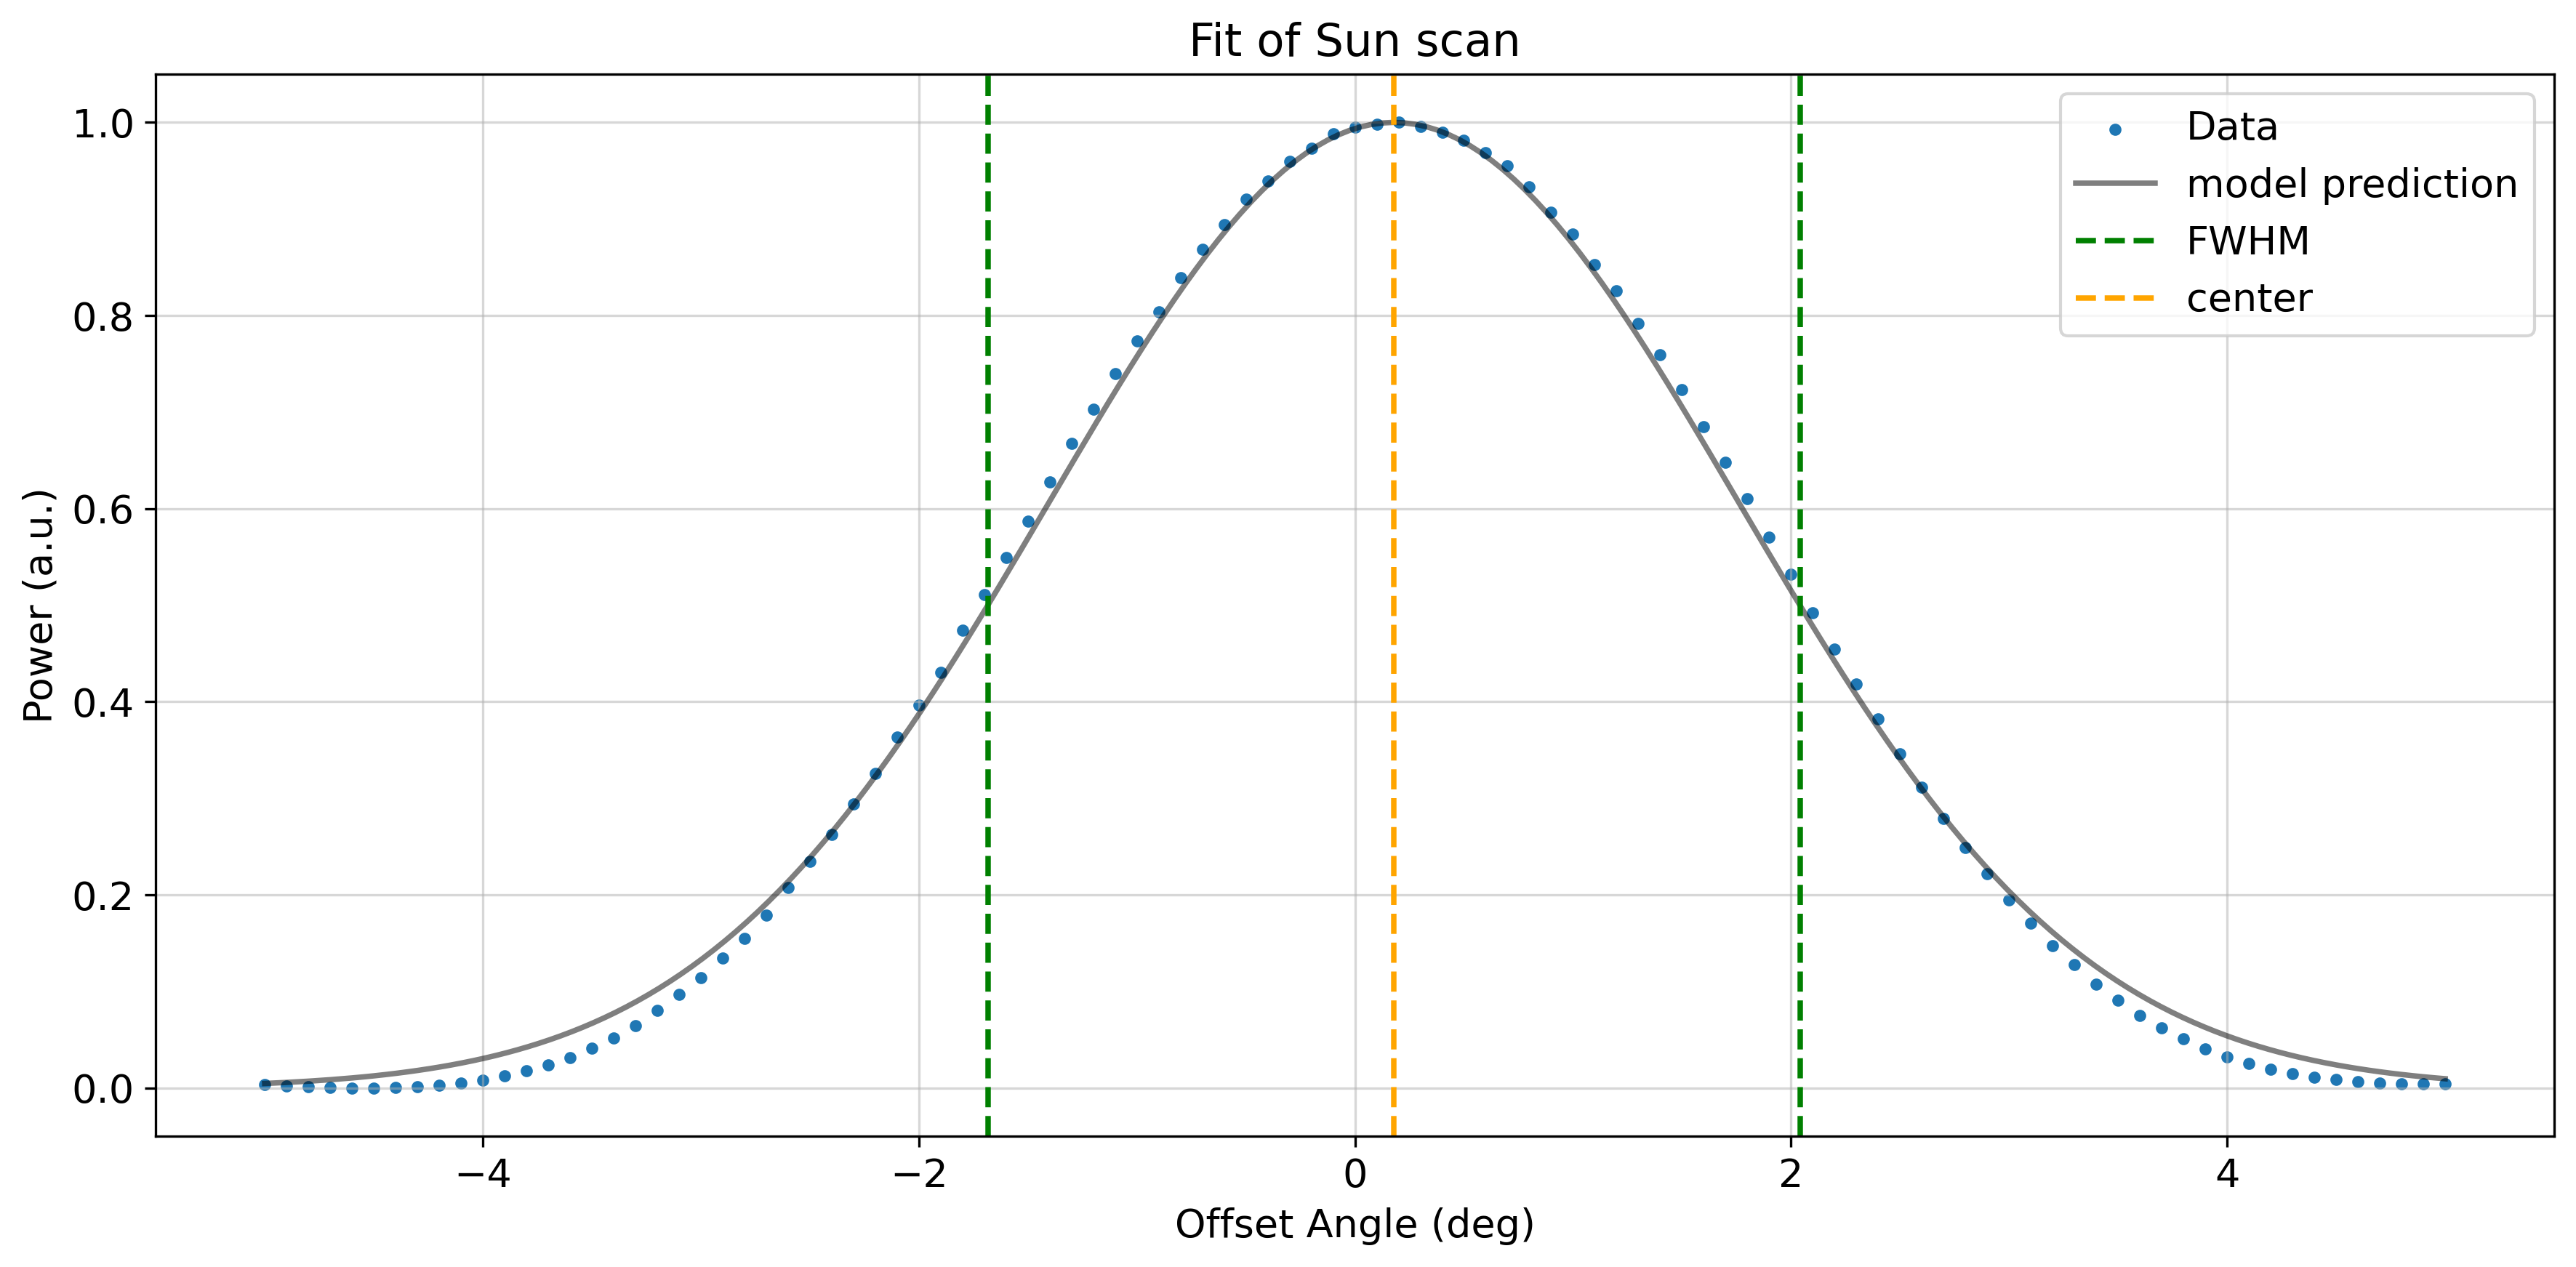
\includegraphics[width=\textwidth]{assets/sun_scan_fit_h.png}
        \caption{Fit to the horizontal scan}
        \label{fig:sun_fit_h}
    \end{subfigure}
    \hfill
    \begin{subfigure}[b]{0.45\textwidth}
        \centering
        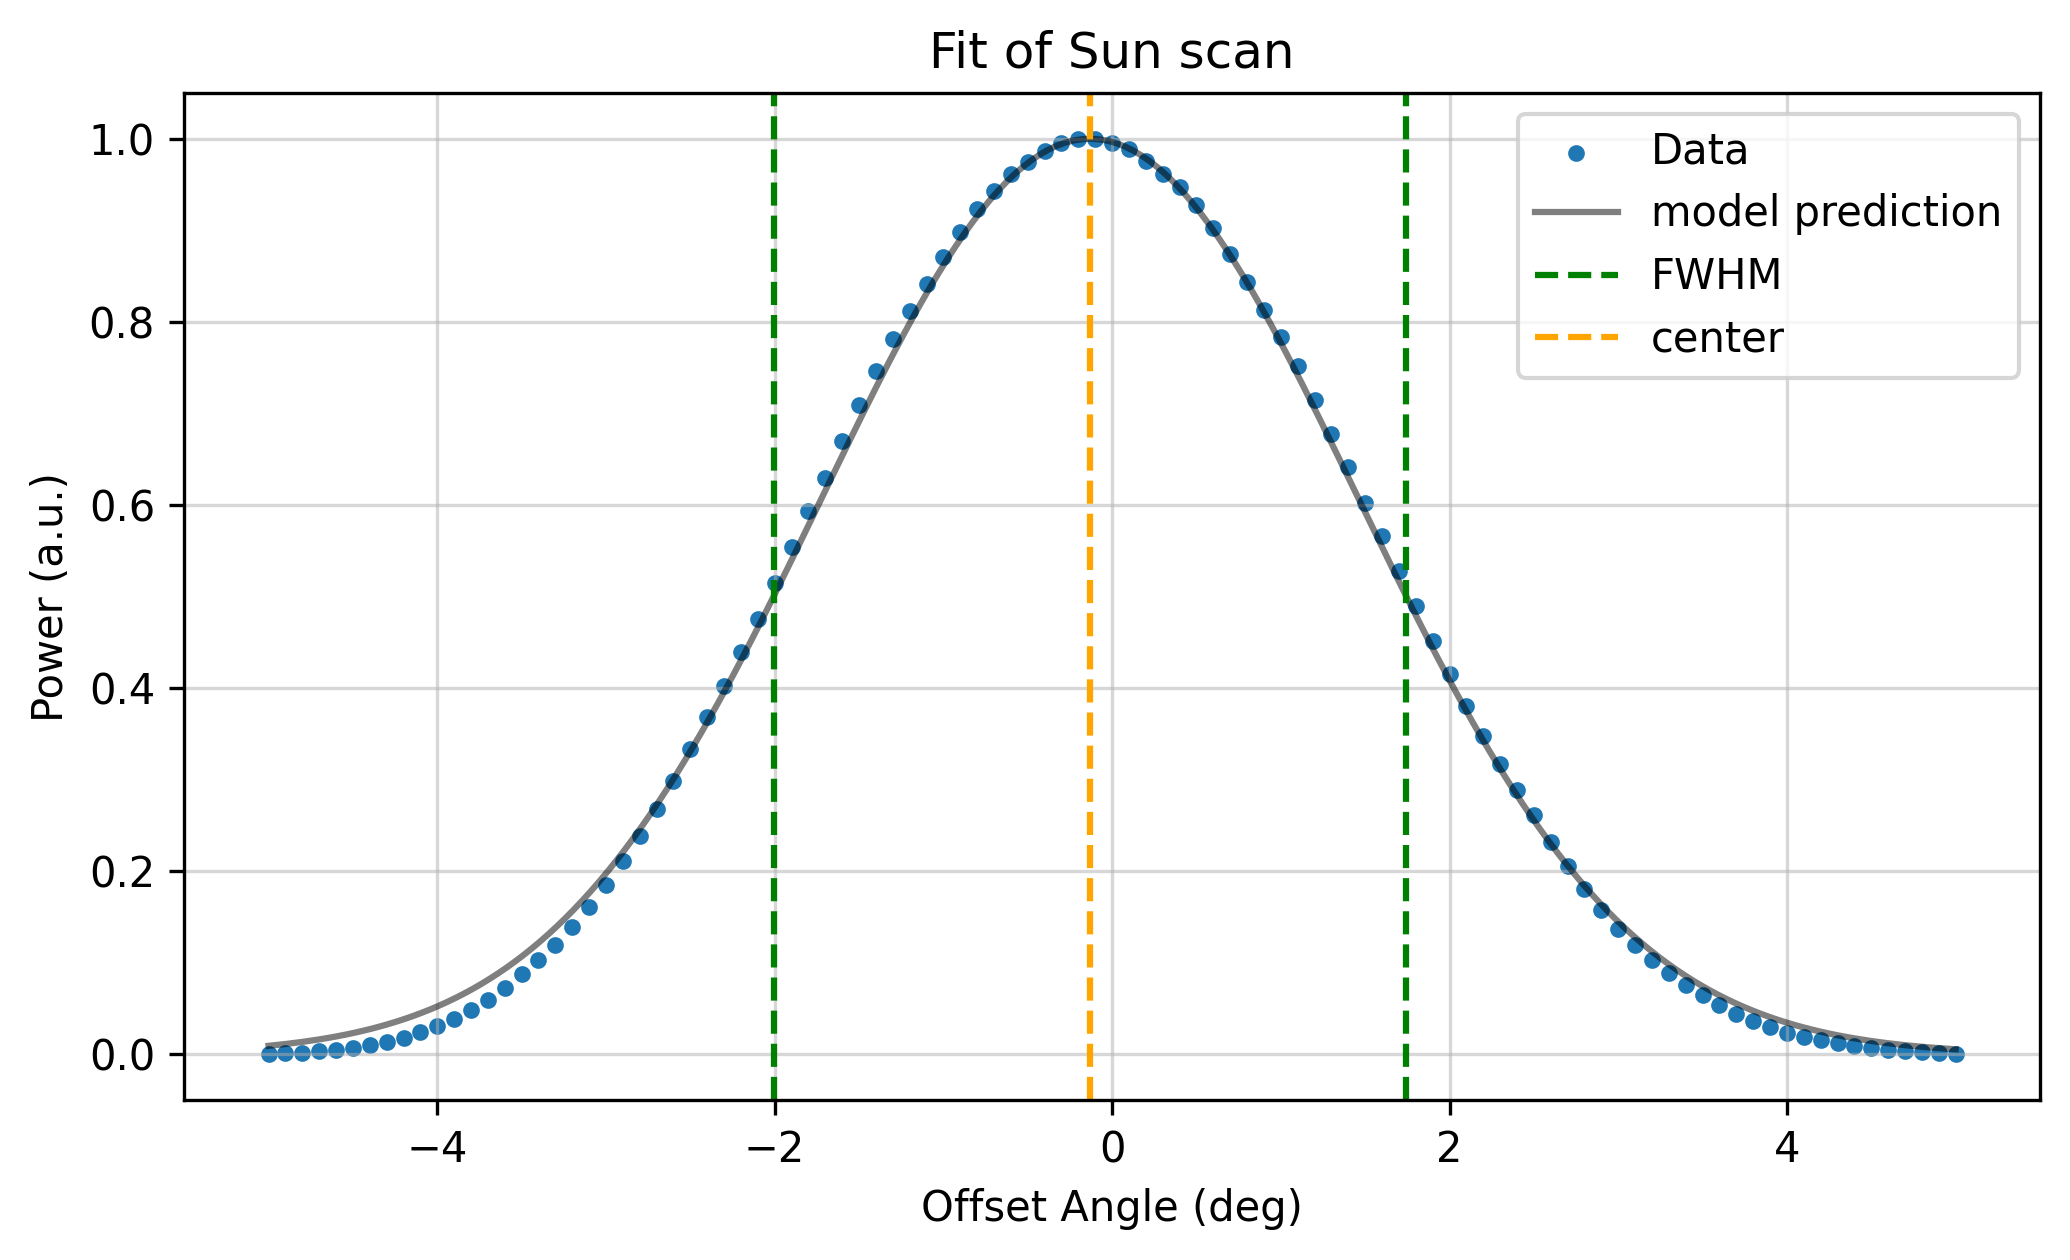
\includegraphics[width=\textwidth]{assets/sun_scan_fit_v.png}
        \caption{Fit to the vertical scan}
        \label{fig:sun_fit_v}
    \end{subfigure}
    \caption{Iterative least squares fits to the sun scans}
    \label{fig:sun_scan_fit}
\end{figure}

We can also compute the average FWHM $= \SI{3.738(0.008)}{\degree}$, which will be used for further calculations.
If we compare the values for the FWHM from table \ref{tab:params} with those from table \ref{tab:ang_res}
we find that the theoretical values do not lie within the error bounds of the measured value.
We think the reason for this discrepancy is a combination of

\begin{itemize}
    \item Unknown errors in the given constants $d = \SI{4}{m}$ and $\eta = 0.5$, especially $\eta$ since it is not trivial to measure.
    \item Invalid assumption that the main lobe is gaussian.
    \item Invalid assumption that the solid angle that is not in the main lobe is negligible.
    \item Invalid assumption that the contribution from the integral in Eq. \eqref{eq:gauss_integral} of the gaussian with $\theta > \pi$ is negligible.
\end{itemize}

Of these we think that the uncertainty in $\eta$ has the biggest contribution to the error. Using Eq. \eqref{eq:fwhm}, the average FWHM, a carrier frequency of \SI{1.4204}{\giga \hertz} and antenna diameter of \SI{4}{m}
We can compute an inferred antenna efficiency which would be consistent with our measurements. This would have a value of $\eta = \SI{0.735(0.003)}{}$.

The pointing offset, i.e. the difference between the optical direction of the telescope and the geometrical direction can also be simply read from these fits, as the values of $\theta_0$ in the horizontal and vertical directions.
TODO: figure out in which direction the telescope would need to be adjusted, i don't understand the coordinate system enough for that :(